
\documentclass[oneside]{diretrizes}            % Imprimir apenas frente
%\documentclass[doubleside]{diretrizes}        % Imprimir frente e verso
% Importações de pacotes
\usepackage[alf, abnt-emphasize=bf, recuo=0cm, abnt-etal-cite=2, abnt-etal-list=0]{abntex2cite}  % Citações padrão ABNT
\usepackage[utf8]{inputenc}                         % Acentuação direta
\usepackage[T1]{fontenc}                            % Codificação da fonte em 8 bits
\usepackage{graphicx}                               % Inserir figuras
\usepackage{amsfonts, amssymb, amsmath}             % Fonte e símbolos matemáticos
\usepackage{booktabs}                               % Comandos para tabelas
\usepackage{verbatim}                               % Texto é interpretado como escrito no documento
\usepackage{multirow, array}                        % Múltiplas linhas e colunas em tabelas
\usepackage{indentfirst}                            % Endenta o primeiro parágrafo de cada seção.
\usepackage{microtype}                              % Para melhorias de justificação?
\usepackage[algoruled, portuguese]{algorithm2e}     % Escrever algoritmos
\usepackage{float}                                  % Utilizado para criação de floats
\usepackage{times}                                  % Usa a fonte Times
\usepackage{color}
\usepackage{listings}
\usepackage{xcolor}

\definecolor{codegreen}{rgb}{0,0.6,0}
\definecolor{black}{rgb}{0,0,0}
\definecolor{codegray}{rgb}{0.5,0.5,0.5}
\definecolor{lightgray}{rgb}{0.8,0.8,0.8}
\definecolor{codepurple}{rgb}{0.58,0,0.82}
\definecolor{backcolour}{rgb}{0.95,0.95,0.92}

\renewcommand{\lstlistingname}{Código} % Mudar o nome de "Listing"

\lstdefinestyle{mystyle}{
    backgroundcolor=\color{backcolour},
    commentstyle=\color{codegreen},
    keywordstyle=\color{magenta},
    numberstyle=\tiny\color{codegray},
    stringstyle=\color{codepurple},
    basicstyle=\ttfamily\footnotesize,
    breakatwhitespace=false,
    breaklines=true,
    captionpos=b,
    keepspaces=true,
    numbers=left,
    numbersep=5pt,
    showspaces=false,
    showstringspaces=false,
    showtabs=false,
    tabsize=2
}

\lstdefinestyle{bash}{
    backgroundcolor=\color{black},
    commentstyle=\color{codegreen},
    keywordstyle=\color{codegray},
    numberstyle=\tiny\color{codegray},
    stringstyle=\color{lightgray},
    basicstyle=\ttfamily\footnotesize\color{white},
    breakatwhitespace=false,
    breaklines=true,
    captionpos=b,
    keepspaces=true,
    numbers=left,
    numbersep=5pt,
    showspaces=false,
    showstringspaces=false,
    showtabs=false,
    xleftmargin=0pt
}


\lstset{style=mystyle}

% Inclui o preâmbulo do documento
\usepackage{helvet}
\renewcommand{\familydefault}{\sfdefault}

\instituicao{Universidade do Vale do Itajaí}
\abreviatura{UNIVALI}
\departamento{Campus Itajaí}
\localapresentacao{Itajaí}
\nomeautor{Ian Callegari Aragão, Lucas Losekann Rosa e Lucas Carvalho de Borba}
\titulotb{Projeto de Sistemas Distribuídos: Chat Distribuído}
%\subtitulo{Subtítulo do trabalho}
\anoapresentacao{2026}
\dataapresentacao{09 de Setembro de 2026}
\mesapresentacao{Setembro}




\usepackage[a4paper, top=3.0cm, bottom=2.0cm, left=3.0cm, right=2.0cm]{geometry} %teste margem
%\usepackage{titlesec} %teste margem

\newcommand{\blue}[1]{\textcolor{blue}{#1}} % proposed
\newcommand{\red}[1]{\textcolor{red}{#1}} % to be removed
\newcommand{\green}[1]{\textcolor{green}{#1}} % to be discussed?
\newcommand{\yellow}[1]{\textcolor{yellow}{#1}} % ????
\newcommand{\magenta}[1]{\textcolor{magenta}{#1}} % warning - requires attention

% Define as cores dos links e informações do PDF
\makeatletter
\hypersetup{
    portuguese,
    colorlinks,
    linkcolor=black,
    citecolor=black,
    filecolor=black,
    urlcolor=black,
    breaklinks=true,
    pdftitle={\@title},
    pdfauthor={\@author},
    pdfsubject={\imprimirpreambulo},
    pdfkeywords={abnt, latex, abntex, abntex2}
}
\makeatother

% Redefinição de labels
\renewcommand{\algorithmautorefname}{Algoritmo}
\def\equationautorefname~#1\null{Equa\c c\~ao~(#1)\null}

% Cria o índice remissivo
\makeindex

% Início do documento
\begin{document}

    % Retira espaço extra obsoleto entre as frases.
    \frenchspacing
    % Elementos pré textuais
    \pretextual
    \include{./01-elementos-pre-textuais/capa}              % Capa
    %
% Documento: FOLHA DE ROSTO
%

\makeatletter
\begin{folhaderosto}
	\thispagestyle{empty}%limpa estilo da pagina
	
    \begin{center}
    
		\small\textbf{\expandafter\uppercase\expandafter{\imprimirnomeautor}}\\
		\vspace*{6.2 cm}%Espaço entre linhas
		\normalsize\textbf{\expandafter\uppercase\expandafter{\imprimirtitulotb}}\\
		
    \end{center}
	
	\vspace*{2.35 cm}%Espaçamento entre linhas
		    \large%tamanho da fonte 
    		\hfill%Estica horizontamente  com espaços
	    	\begin{minipage}{8 cm}%Minipagina
	    		\begin{small} %Muda tamanho da fonte
	    		\setlength{\baselineskip}{0.7\baselineskip}
				
		    	{Trabalho da M2 do Curso de Ciência da Computação,
		    	da matéria de Sistemas Operacionais da {\imprimirinstituicao},
		    	ministrada pelo Professor Felipe Viel.
		    	}
				
				
				\end{small} %Muda tamanho da fonte
		    \end{minipage}%%Minipagina
		    	
		    \vspace*{6 cm}%Espaçamento entre linhas
		    
		    \begin{center} %Alinhamento centralizado
		    	\normalsize %Muda tamanho da fonte
	    		\textbf{\imprimirlocalapresentacao, \imprimirdataapresentacao}
	    	\end{center}%Alinhamento centralizado

\end{folhaderosto}
\makeatother
        % Folha de rosto

    %
% Documento: Resumo (Português)
%

\begin{RESUMO}
\thispagestyle{empty}

    \noindent Este relatório apresenta o desenvolvimento de um chat distribuído
    executado por processos independentes e comunicado exclusivamente por sockets
    TCP. A solução permite configurar até 15 nós a partir de um catálogo estático
    de endereços, mantém relógios vetoriais e utiliza um nó coordenador como
    sequenciador das mensagens de grupo. Cada mensagem de grupo recebe um número
    de sequência global e é difundida por unicast a todos os participantes; em
    cada receptor, um buffer somente libera sequências contíguas. Também foram
    implementados detecção de falhas por batimentos periódicos e reeleição do
    coordenador pelo algoritmo do Valentão. Ensaios automatizados com sockets reais
    em uma única máquina, envolvendo 3, 8 e 15 processos independentes, confirmaram que
    todos os nós ativos entregaram as mensagens de grupo na mesma ordem e sem itens
    remanescentes no buffer. A análise do código e um ensaio de falha também
    identificaram limitações do protótipo: o recebimento de mensagens privadas, a
    captura de estado global e a continuidade do contador global após a troca de
    líder ainda não estão concluídos. Essas lacunas são documentadas para separar
    os requisitos demonstrados daqueles que dependem de evolução da implementação.

    \vspace*{0.5cm}\noindent\textbf{Palavras-chave}: sistemas distribuídos;
    comunicação de grupo; ordem total; relógio vetorial; eleição de líder.

\end{RESUMO}


    \sumario
\begin{OnehalfSpacing}

    % Elementos textuais
    \textual
    %
% Documento: Introdução
%
\chapter{INTRODUÇÃO}\label{chap:introducao}

Sistemas distribuídos são formados por processos independentes que cooperam por
troca de mensagens. Como não há memória nem relógio físico compartilhados, a
observação de eventos e a manutenção de uma ordem comum exigem protocolos
explícitos. Relógios lógicos preservam relações de precedência, enquanto relógios
vetoriais permitem representar relações causais e identificar eventos concorrentes
\cite{lamport1978,tanenbaum2007}. Ainda assim, causalidade define apenas uma ordem
parcial: mensagens concorrentes podem ser observadas em ordens diferentes por
participantes distintos.

O trabalho propõe a implementação de uma aplicação distribuída com comunicação de
grupo, ordem total, número configurável de nós, interface por nó e captura de um
estado global consistente. Entre os temas oferecidos, escolheu-se o
\textbf{chat distribuído}. Cada participante é um processo do sistema operacional,
com estado privado e endereço próprio. A única informação compartilhada antes da
execução é o catálogo estático de endereços; durante a execução, toda coordenação
ocorre por mensagens de rede.

Para estabelecer uma sequência única das mensagens de grupo, foi escolhida a
abordagem de \textbf{sequenciador}. Um coordenador atribui números globais
monotônicos e redifunde as mensagens; relógios vetoriais permanecem anexados aos
eventos para registrar a evolução causal. Como o coordenador é um ponto crítico,
o protótipo emprega batimentos de saúde e o algoritmo do Valentão para eleição de
um substituto. Essa opção reduz a complexidade do caminho normal de entrega, ao
custo de exigir tratamento cuidadoso para a falha do líder.

O objetivo deste relatório é descrever fielmente a arquitetura encontrada no
repositório, explicar seus algoritmos e registrar os resultados verificáveis. Por
isso, além das funcionalidades demonstradas, são apresentadas as limitações ainda
existentes. Em especial, a versão analisada não implementa a captura de estado
global e não conclui o recebimento de mensagens privadas, embora a interface de
envio já exista.

\section{Organização do relatório}

O Capítulo~\ref{chap:projeto} descreve equipe, tecnologias, arquitetura, rede e
execução. O Capítulo~\ref{chap:algoritmos} detalha relógio vetorial, ordem total,
eleição e a alternativa planejada para estado global. O
Capítulo~\ref{chap:avaliacao} apresenta os cenários de validação e as limitações.
Por fim, o Capítulo~\ref{chap:conclusao} sintetiza os resultados e os requisitos
pendentes.
            % Introdução
    \chapter{PROJETO E ARQUITETURA}\label{chap:projeto}

\section{Tema e escopo}

A aplicação representa um bate-papo no qual cada nó corresponde a um
participante. O escopo implementado prioriza o middleware: inicialização de
múltiplos processos, serialização das mensagens, comunicação ponto a ponto,
difusão ao grupo, registro das ordens local e global, relógio vetorial,
monitoramento, eleição e \textit{snapshot} distribuído. A interface é textual,
suficiente para observar os estados internos relevantes ao experimento.

O número de nós é informado em tempo de execução. O arquivo
\texttt{json/nodes.json} contém 15 entradas, e cada processo lê apenas as
primeiras $N$. Portanto, a configuração entregue suporta de 1 a 15 nós sem
alteração do código ou do arquivo de endereços, atendendo ao limite mínimo
solicitado pelo roteiro.

\section{Participação da equipe}

A divisão apresentada na Tabela~\ref{tab:equipe} foi construída a partir do
histórico de commits do repositório no \textit{GitHub}, mas as atividades de
integração, revisão, validação e criação do relatório foram conduzidas em
conjunto. Ademais, a partipação ativa do integrante, Lucas Carvalho de Borba,
no desenvolvimento foi reduzida devido a sua presença no evento \textit{LASC
    (Latin American Space Challenge)}.

\begin{table}[H]
    \centering
    \caption{Participação dos integrantes}
    \label{tab:equipe}
    \begin{tabular}{p{4.5cm} p{10.0cm}}
        \toprule
        \textbf{Integrante}     & \textbf{Principais contribuições}                \\
        \midrule
        Ian Callegari Aragão    & Configuração inicial; servidor e comunicação por
        sockets; tratamento de comandos; relógio vetorial; \text{health-check},
        estados dos nós e ajustes na eleição.                                      \\\\

        Lucas Losekann Rosa     & Interface de terminal e script de inicialização;
        mecanismo de ordenação e buffer de entrega; implementação e correções da
        eleição de líder; implementação do algorítimo de \textit{Chandy-Lamport}.  \\\\

        Lucas Carvalho de Borba & Testes na aplicação, validação dos requisitos e
        suporte na construção do relatório.                                        \\ \bottomrule
    \end{tabular}
\end{table}

\section{Tecnologias utilizadas}

A implementação foi escrita em Python 3.10 ou superior. O projeto é gerenciado
por \texttt{uv}, enquanto a comunicação, concorrência e serialização usam
principalmente módulos da biblioteca padrão: \texttt{socket},
\texttt{threading}, \texttt{json}, \texttt{dataclasses}, \texttt{argparse} e
\texttt{signal}. A rede é implementada diretamente sobre sockets TCP e a
interface usa sequências ANSI no terminal.

\section{Componentes da solução}

A Tabela~\ref{tab:componentes} relaciona as principais unidades do projeto.

\begin{table}[H]
    \centering
    \caption{Componentes do protótipo}
    \label{tab:componentes}
    \begin{tabular}{p{5.0 cm} p{10.0cm}}
        \toprule
        \textbf{Componente}           & \textbf{Responsabilidade}                          \\
        \midrule
        \texttt{lauch\_node.py}       & Lê os argumentos \texttt{--id} e
        \texttt{--count}, carrega o catálogo e instancia um nó.                            \\\\

        \texttt{services/node.py}     & Mantém relógios, históricos, buffer,
        sequências, estado dos pares, interface de comandos, heartbeat, eleição,
        recuperação da ordem e coordenação do snapshot.                                    \\\\

        \texttt{services/socket.py}   & Abre o servidor TCP, aceita conexões e envia
        documentos JSON.                                                                   \\\\

        \texttt{services/terminal.py} & Mantém uma área de rolagem e uma linha
        fixa de entrada para a interface textual.                                          \\\\

        \texttt{models/node\_dto.py}  & Define o formato lógico das mensagens.             \\\\

        \texttt{models/snapshot\_ses-}                                                     \\ \texttt{-sion.py} & Mantém os canais em gravação,
        estados de canal e relatórios de uma captura.                                      \\\\

        \texttt{json/nodes.json}      & Catálogo estático com IDs, endereço IP e portas.   \\\\

        \texttt{start.sh}             & Abre $N$ processos em terminais Konsole separados. \\\\

        \bottomrule
    \end{tabular}
\end{table}

Cada nó possui memória privada. Dentro do processo, três fluxos concorrentes
são iniciados: escuta TCP, emissão periódica de batimentos (\textit{heartbeat})
e verificação de saúde (\textit{health-check}). A interface é executada no
fluxo principal. Locks distintos protegem relógio vetorial, histórico local,
contador do sequenciador, entrega, heartbeat e eleição.

\begin{figure}[H]
    \centering
    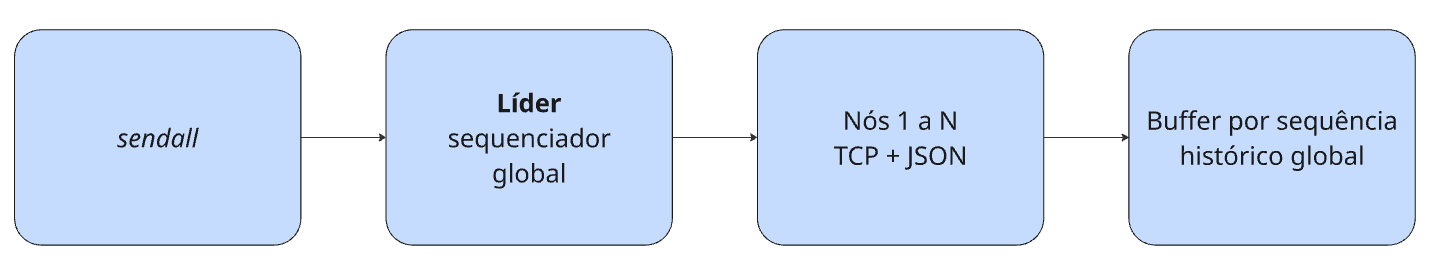
\includegraphics[width=1.0\textwidth]{04-figuras/fluxo_sendall.png}
    \caption{Fluxo de uma mensagem de grupo}
    \label{fig:arquitetura}
\end{figure}

\section{Formato e fluxo das mensagens}

As mensagens são serializadas como objetos JSON derivados de \texttt{NodeDto}.
Os campos comuns são: tipo, origem, horário, relógio vetorial e texto. Conforme
a operação, também são informados destino, sequência local e sequência global.
Os tipos declarados incluem mensagem privada, pedido de mensagem de grupo,
mensagem de grupo ordenada, heartbeat, confirmação de heartbeat, eleição,
coordenador, atualização da lista de nós, marcador e relatório de snapshot,
pedido e resposta de estado da ordem global. Os campos \texttt{channel\_origin}
e \texttt{channel\_sequence} identificam o emissor TCP e a posição da mensagem
no canal lógico sem confundi-lo com o autor original de uma mensagem
retransmitida pelo líder.

Em cada envio, \texttt{Socket.send} abre uma conexão TCP, transmite um
documento JSON e fecha a conexão. O receptor aceita a conexão, lê blocos de até
65.536 bytes até o fechamento do emissor e então delega o documento completo ao
nó \cite{python-socket}. A escolha por unicast TCP foi motivada pela entrega
confiável e pela simplicidade de endereçamento em uma única máquina. Para
difusão, o líder itera sobre o catálogo e envia uma cópia para cada
participante. Em comparação ao multicast UDP, essa solução evita implementar
confirmação e retransmissão de datagramas. 

Além disso, o multicast UDP não
oferece, por si só, um mecanismo específico para comunicação privada entre dois
participantes, sendo necessária a implementação de uma lógica adicional para
distinguir e encaminhar mensagens privadas. Com TCP unicast, essa distinção é
obtida naturalmente pelo endereço do destinatário da conexão, não sendo
necessário implementar um mecanismo adicional de comunicação privada. Como
contrapartida, a difusão realiza $N$ entregas por mensagem de grupo e concentra
esse custo no coordenador.

\section{Endereçamento}

Todos os ensaios foram executados pela interface de loopback, de modo que a
rede não sai da máquina local. Cada nó possui uma porta exclusiva, conforme a
Tabela~\ref{tab:enderecos}. O servidor escuta em \texttt{0.0.0.0}, enquanto o
catálogo usa \texttt{127.0.0.1} como destino.

\begin{table}[H]
    \centering
    \caption{Catálogo de endereços da simulação}
    \label{tab:enderecos}
    \setlength{\tabcolsep}{3pt}
    \small
    \begin{tabular}{ccc@{\hspace{0.6cm}}ccc@{\hspace{0.6cm}}ccc}
        \toprule
        \textbf{Nó} & \textbf{IP} & \textbf{Porta} &
        \textbf{Nó} & \textbf{IP} & \textbf{Porta} &
        \textbf{Nó} & \textbf{IP} & \textbf{Porta}                                                 \\
        \midrule
        1           & 127.0.0.1   & 5001           & 6  & 127.0.0.1 & 5006 & 11 & 127.0.0.1 & 5011 \\
        2           & 127.0.0.1   & 5002           & 7  & 127.0.0.1 & 5007 & 12 & 127.0.0.1 & 5012 \\
        3           & 127.0.0.1   & 5003           & 8  & 127.0.0.1 & 5008 & 13 & 127.0.0.1 & 5013 \\
        4           & 127.0.0.1   & 5004           & 9  & 127.0.0.1 & 5009 & 14 & 127.0.0.1 & 5014 \\
        5           & 127.0.0.1   & 5005           & 10 & 127.0.0.1 & 5010 & 15 & 127.0.0.1 & 5015 \\
        \bottomrule
    \end{tabular}
\end{table}

\section{Interface e execução}

O script automático depende de Linux, \texttt{bash}, \texttt{setsid},
\texttt{Konsole} e \texttt{uv}. Na raiz do repositório, a inicialização de
três, oito ou quinze nós é feita por:

\begin{lstlisting}[style=bash, numbers=none]
./start.sh --count <quantidade>
\end{lstlisting}

Também é possível abrir terminais manualmente e executar um processo em cada
um:

\begin{lstlisting}[style=bash, numbers=none]
uv run python lauch_node.py --id <identificador> --count <quantidade>
\end{lstlisting}

Os comandos da interface são descritos na Tabela~\ref{tab:comandos}.

\begin{table}[H]
    \centering
    \caption{Comandos disponíveis em cada nó}
    \label{tab:comandos}
    \begin{tabular}{p{4.5cm} p{9.5cm}}
        \toprule
        \textbf{Comando}              & \textbf{Função}                                          \\
        \midrule
        \texttt{send ID mensagem}     & Envia uma mensagem privada ao endereço do ID.            \\
        \texttt{sendall mensagem}     & Solicita ao líder a ordenação e difusão ao grupo.        \\
        \texttt{local}                & Exibe os envios produzidos localmente e sua sequência.   \\
        \texttt{global}               & Exibe as mensagens de grupo já entregues em ordem total. \\
        \texttt{status}               & Exibe líder, vetor, próxima sequência e históricos.      \\
        \texttt{list}                 & Exibe endereço e estado ativo/inativo dos participantes. \\
        \texttt{snapshot}             & Inicia \textit{Chandy-Lamport} e exibe o estado global após
        receber os fragmentos dos nós ativos.                                                    \\
        \texttt{help} & Lista os comandos disponíveis.                                            \\
        \texttt{exit} & Encerra o processo.                                                       \\
        \bottomrule
    \end{tabular}
\end{table}

No comando \texttt{send}, somente o emissor registra o evento em sua ordem
local. O documento \texttt{PRIVATE\_MESSAGE} é encaminhado ao endereço do
destino, que combina o vetor recebido com o seu relógio, incrementa a própria
posição e exibe a mensagem com o rótulo \texttt{[PRIVADA]}. Como se trata de
unicast, ela não recebe sequência global nem aparece no histórico dos demais
participantes.
               % Projeto e arquitetura
    \chapter{ALGORITMOS DISTRIBUÍDOS}\label{chap:algoritmos}

\section{Relógio vetorial}

Cada nó mantém um vetor $V$ de tamanho $N$. A posição $V[i]$ representa o
conhecimento local sobre os eventos do nó $i$. Ao criar uma mensagem local no nó
$i$, a implementação executa

\begin{equation}
    V[i] \leftarrow V[i] + 1
\end{equation}

e anexa uma cópia do vetor à mensagem. Ao processar um vetor recebido $V_m$, o nó
calcula, componente a componente,

\begin{equation}
    V[j] \leftarrow \max(V[j], V_m[j]), \quad 1 \leq j \leq N,
\end{equation}

e depois incrementa sua própria posição. Essa política é compatível com a
interpretação de recepção como evento local. O uso de vetores permite registrar
mais informação causal que um relógio escalar \cite{coulouris2011}.

Na abordagem adotada, o vetor não decide a ordem total. Ele acompanha pedidos e
mensagens ordenadas para permitir inspeção causal, enquanto o número fornecido
pelo sequenciador é a autoridade para entrega. Portanto, a solução corresponde à
abordagem B do roteiro.

\section{Ordem total por sequenciador}\label{sec:ordem-total}

O líder inicial é configurado como o nó 1. Uma mensagem de grupo percorre as
etapas a seguir:

\begin{enumerate}
    \item O emissor incrementa sua posição no relógio vetorial, incrementa o
    contador de ordem local e armazena o envio no histórico local.
    \item Se o emissor não é o líder, abre uma conexão TCP com o coordenador e
    envia um \texttt{GROUP\_MESSAGE\_REQUEST}. Se é o líder, chama diretamente a
    rotina de sequenciamento.
    \item O líder protege \texttt{next\_global\_sequence} com um lock, atribui seu
    valor à mensagem e incrementa o contador.
    \item A mensagem passa a ter o tipo \texttt{ORDERED\_GROUP\_MESSAGE} e é
    enviada individualmente a todos os nós. A cópia do próprio líder é tratada
    localmente.
    \item Cada receptor indexa a mensagem por sua sequência no buffer. Sequências
    menores que a próxima esperada são descartadas como duplicatas antigas.
    \item Enquanto a próxima sequência esperada estiver presente, o receptor a
    remove do buffer, atualiza o relógio vetorial, acrescenta a mensagem ao
    histórico global e avança a sequência esperada.
\end{enumerate}

O buffer é necessário porque conexões TCP diferentes não estabelecem ordem entre
si. Assim, mesmo que a mensagem 4 chegue antes da 3, ela permanece retida até que
a lacuna seja preenchida. Como todos recebem os mesmos números e aplicam a mesma
regra de liberação, os históricos convergem para a mesma ordem.

\subsection{Exemplo numérico com mensagens concorrentes}

Considere três nós com vetores inicialmente iguais a $[0,0,0]$. O nó 2 cria a
mensagem A e a carimba com $[0,1,0]$; concorrentemente, o nó 3 cria B com
$[0,0,1]$. Nenhum vetor é componente a componente menor que o outro, portanto A e
B são concorrentes. Suponha que o líder receba B antes de A. Ele atribui os números
globais mostrados na Tabela~\ref{tab:exemplo-ordem}.

\begin{table}[H]
    \centering
    \caption{Sequenciamento de duas mensagens concorrentes}
    \label{tab:exemplo-ordem}
    \begin{tabular}{ccccc}
        \toprule
        \textbf{Mensagem} & \textbf{Origem} & \textbf{Vetor} &
        \textbf{Ordem local} & \textbf{Ordem global} \\
        \midrule
        B & 3 & $[0,0,1]$ & 1 & 1 \\
        A & 2 & $[0,1,0]$ & 1 & 2 \\
        \bottomrule
    \end{tabular}
\end{table}

Se A, de sequência 2, chegar primeiro ao nó 1, ela aguarda no buffer. Quando B
chega com sequência 1, o nó entrega B e, em seguida, A. O mesmo ocorre no nó 2:

\begin{equation}
    H_1 = H_2 = \langle (1,B), (2,A) \rangle.
\end{equation}

O exemplo mostra que o vetor identifica a concorrência, mas é a decisão do
sequenciador que transforma as mensagens em uma ordem total.

\section{Monitoramento e eleição de líder}\label{sec:eleicao}

O coordenador envia uma mensagem \texttt{HEARTBEAT} a cada nó ativo a cada cinco
segundos. O receptor responde com \texttt{HEARTBEAT\_ACK}. O líder registra o
instante da última confirmação, enquanto os seguidores registram o último
batimento do coordenador. O limiar base é de dez segundos e a inativação ou
eleição ocorre após três verificações vencidas. Quando o líder considera um
participante inativo, difunde uma atualização da lista.

A eleição segue o algoritmo do Valentão. Seu passo a passo na implementação é:

\begin{enumerate}
    \item O nó que detecta a indisponibilidade marca o líder anterior como inativo
    e envia \texttt{ELECTION} a cada nó ativo de ID maior.
    \item Uma conexão bem-sucedida é tratada como indicação de que o nó superior
    continuará a eleição. Ao receber a solicitação, todo nó de ID superior inicia
    sua própria rodada.
    \item Um participante sem nó superior acessível declara-se coordenador.
    \item O vencedor difunde \texttt{COORDINATOR}; os receptores atualizam
    \texttt{leader\_id} e encerram o estado local de eleição.
\end{enumerate}

Consequentemente, o maior ID ativo alcançado vence, conforme a propriedade do
algoritmo do Valentão \cite{tanenbaum2007}. A implementação simplifica o protocolo:
não há mensagem \texttt{OK} separada nem timeout específico para aguardar o anúncio;
o sucesso da conexão de eleição exerce o papel da confirmação.

\section{Estado global: escolha e situação atual}\label{sec:estado-global}

Um estado global reúne os estados locais e as mensagens em trânsito de modo
compatível com a causalidade. O algoritmo de Chandy--Lamport é uma escolha adequada
porque não exige relógio físico sincronizado nem a interrupção da aplicação; por
meio de marcadores, ele registra um corte consistente da execução
\cite{chandy1985}.

Para este projeto, a implementação planejada deveria seguir estas etapas:

\begin{enumerate}
    \item O iniciador registra relógio vetorial, líder, histórico local, histórico
    global, próxima sequência esperada e estado dos participantes; depois envia um
    marcador a todos os canais de saída.
    \item Ao receber o primeiro marcador, cada nó registra o próprio estado, marca
    o canal de chegada como vazio e encaminha marcadores aos demais nós.
    \item Até receber o marcador de cada origem, o nó registra como estado daquele
    canal as mensagens de aplicação recebidas após seu estado local.
    \item Cada nó envia o fragmento concluído ao iniciador, que agrega e exibe o
    snapshot.
\end{enumerate}

Entretanto, a versão analisada não declara mensagens de marcador, não mantém
sessões de snapshot e não oferece comando para iniciar ou exibir a captura. Logo,
o requisito de estado global ainda \textbf{não está implementado}. Além disso, o
transporte abre uma nova conexão TCP por documento. Embora TCP seja FIFO dentro de
uma conexão, conexões distintas entre o mesmo par não formam automaticamente um
canal FIFO único. Uma implementação correta de Chandy--Lamport deve manter
conexões persistentes por par ou numerar mensagens e marcadores por canal antes de
aplicar o protocolo.
            % Algoritmos distribuídos
    \chapter{AVALIAÇÃO EXPERIMENTAL}\label{chap:avaliacao}

\section{Metodologia}

Foram executados ensaios temporários sobre o código do repositório, sem modificar
a implementação. Cada nó foi iniciado pelo sistema operacional como um processo
separado, usando o ponto de entrada \texttt{lauch\_node.py}, o catálogo original e
as portas 5001 a 5015 em \texttt{127.0.0.1}. Os comandos foram escritos na entrada
padrão dos processos em rápida sucessão e percorreram sockets TCP reais. Depois
das entregas, o comando \texttt{global} foi solicitado em todos os terminais; as
tuplas (sequência global, origem, texto) foram extraídas das saídas e comparadas.
Todos os processos encerraram normalmente.

Não há arquivos-fonte de testes no diretório \texttt{tests} da versão avaliada;
foi encontrado apenas um arquivo \texttt{.pyc} antigo. O comando
\texttt{uv run pytest} também não pôde ser usado porque \texttt{pytest} não está
declarado nas dependências. Por esse motivo, os resultados desta seção provêm do
ensaio externo descrito acima.

\section{Ordem global com 3, 8 e 15 nós}

Os três cenários foram concluídos com todos os históricos idênticos e todos os
buffers vazios, conforme a Tabela~\ref{tab:testes-ordem}. No ensaio com três nós,
cada participante emitiu uma mensagem. Nos ensaios com oito e quinze, cinco nós
emitiram simultaneamente.

\begin{table}[H]
    \centering
    \caption{Resultados da difusão e entrega ordenada}
    \label{tab:testes-ordem}
    \begin{tabular}{ccccc}
        \toprule
        \textbf{Nós} & \textbf{Envios} & \textbf{Todos receberam} &
        \textbf{Históricos idênticos} & \textbf{Buffers vazios} \\
        \midrule
        3  & 3 & Sim & Sim & Sim \\
        8  & 5 & Sim & Sim & Sim \\
        15 & 5 & Sim & Sim & Sim \\
        \bottomrule
    \end{tabular}
\end{table}

A saída resumida do cenário de 15 nós foi:

\begin{lstlisting}[numbers=none]
GLOBAL 1 | Node 1 | processo-1
GLOBAL 2 | Node 3 | processo-3
GLOBAL 3 | Node 2 | processo-2
GLOBAL 4 | Node 4 | processo-4
GLOBAL 5 | Node 5 | processo-5

comparacao dos 15 historicos: IDENTICOS
buffers restantes: [[], [], [], [], [], [], [], [], [], [], [], [], [], [], []]
\end{lstlisting}

Os pedidos dos nós 2 e 3 foram emitidos em rápida sucessão por processos
independentes, mas o líder aceitou o pedido do nó 3 primeiro. Todos os participantes
observaram a mesma inversão. Isso é uma evidência direta de que a ordem exibida foi
determinada pela sequência global e não por uma suposição local sobre a ordem de
emissão.

\section{Falha e reeleição}

Em um cenário adicional com três nós, duas mensagens foram entregues nas
sequências 1 e 2. Em seguida, o nó 1 foi encerrado e o nó 2 iniciou a eleição. Os
nós 2 e 3 convergiram para o nó 3 como novo líder, demonstrando a seleção do maior
ID ativo. Contudo, a primeira mensagem sequenciada pelo novo líder recebeu
novamente o número 1. Como os receptores sobreviventes já aguardavam a sequência
3, descartaram a mensagem como antiga. O resultado está resumido na
Tabela~\ref{tab:teste-eleicao}.

\begin{table}[H]
    \centering
    \caption{Ensaio de troca do sequenciador}
    \label{tab:teste-eleicao}
    \begin{tabular}{p{8.0cm} p{5.0cm}}
        \toprule
        \textbf{Observação} & \textbf{Resultado} \\
        \midrule
        Histórico antes da falha & $[1,2]$ em todos os nós \\
        Líder eleito entre os nós 2 e 3 & Nó 3 \\
        Primeira sequência criada pelo novo líder & 1 \\
        Próxima sequência esperada nos sobreviventes & 3 \\
        Mensagem posterior entregue & Não \\
        \bottomrule
    \end{tabular}
\end{table}

Assim, a eleição isoladamente funciona no cenário ensaiado, mas a recuperação do
serviço de ordem total não está completa. O novo coordenador precisa recuperar o
maior número estável, por exemplo consultando um quórum de históricos antes de
voltar a sequenciar.

\section{Mensagem privada}

O envio privado do nó 1 para o nó 2 abriu a conexão e retornou sucesso no emissor.
Entretanto, o vetor do receptor permaneceu $[0,0,0]$ e nenhum histórico de recepção
foi produzido. A causa, confirmada pela inspeção de \texttt{handle\_message}, é a
ausência de um ramo para \texttt{PRIVATE\_MESSAGE}. Há ainda uma mensagem de log
rotulada como privada dentro do ramo de mensagem de grupo ordenada. Portanto, o
requisito funcional de conversa privada está apenas parcialmente construído.

\section{Limitações}\label{sec:limitacoes}

Além dos resultados anteriores, a versão atual possui as seguintes limitações:

\begin{itemize}
    \item \textbf{Estado global:} não há comando, marcador nem agregação de
    snapshot; o requisito correspondente permanece pendente.
    \item \textbf{Troca de líder:} contador e histórico do sequenciador não são
    transferidos, interrompendo novas entregas após uma falha que ocorra depois de
    qualquer mensagem já entregue.
    \item \textbf{Mensagem privada:} o emissor envia o documento, mas o receptor
    não trata seu tipo.
    \item \textbf{Relógio vetorial:} em receptores remotos, uma mensagem de grupo
    ordenada atualiza o vetor durante a entrega e novamente no despachante. O líder
    local atualiza apenas uma vez, produzindo políticas de incremento diferentes.
    \item \textbf{Líder inicial:} o nó 1 é fixado como coordenador inicial, mesmo
    que o algoritmo do Valentão normalmente eleja o maior ID ativo.
    \item \textbf{TCP:} cada conexão é lida com uma única chamada de até 65.536
    bytes, sem enquadramento ou laço para remontar documentos maiores. Também não
    há autenticação nem criptografia.
    \item \textbf{Escalabilidade:} uma difusão requer uma conexão por destinatário
    e é feita sequencialmente pelo líder. O catálogo entregue termina no nó 15, e
    \texttt{start.sh} não valida pedidos acima desse limite.
    \item \textbf{Portabilidade:} a inicialização automática depende do terminal
    Konsole e de utilitários típicos de Linux. A execução manual continua possível
    em outros ambientes compatíveis com Python.
    \item \textbf{Testes:} não existe suíte reproduzível em código-fonte no estado
    atual do repositório, nem foram realizados ensaios entre máquinas físicas,
    sob perda de conexão ou com mensagens de grande volume.
\end{itemize}

\section{Síntese dos requisitos}

A Tabela~\ref{tab:requisitos} resume a cobertura verificada. ``Parcial'' indica
que existe uma parte observável do requisito, mas ao menos um cenário obrigatório
ainda falha.

\begin{table}[H]
    \centering
    \caption{Cobertura dos requisitos funcionais}
    \label{tab:requisitos}
    \begin{tabular}{c p{3.3cm} p{8.7cm}}
        \toprule
        \textbf{Req.} & \textbf{Situação} & \textbf{Evidência} \\
        \midrule
        R1 & Atendido & Difusão TCP entregue a todos em 3, 8 e 15 nós. \\
        R2 & Parcial & Chat de grupo funciona; recepção privada está ausente. \\
        R3 & Atendido & Inicialização e entrega verificadas com 3, 8 e 15 processos. \\
        R4 & Parcial & Históricos são idênticos no caminho normal; troca de líder
        perde continuidade da sequência. \\
        R5 & Parcial & Terminal oferece envio, ordens e estado, mas o unicast
        privado não é processado no destino. \\
        R6 & Não atendido & Não há captura nem exibição de estado global. \\
        R7 & Atendido & Itens documentais do roteiro são cobertos neste relatório. \\
        R8 & Parcial & O maior ID ativo é eleito, mas o novo líder não recupera a
        sequência anterior. \\
        \bottomrule
    \end{tabular}
\end{table}
             % Avaliação experimental
    \chapter{CONCLUSÃO}\label{chap:conclusao}

O protótipo demonstra os elementos centrais de comunicação de grupo e ordenação
total em um chat distribuído. Cada participante possui processo, porta e estado
próprios; mensagens de grupo atravessam sockets TCP e recebem uma sequência única
do coordenador. O buffer por lacunas faz com que mensagens recebidas fora de ordem
sejam entregues somente quando todas as posições anteriores estão disponíveis.
Nos ensaios com 3, 8 e 15 nós, todos os participantes terminaram com históricos
globais idênticos e buffers vazios.

O relógio vetorial acompanha as mensagens e torna visível a evolução causal, mas
a ordem total é decidida pelo sequenciador, como previsto pela abordagem B. O
monitoramento por heartbeat e a eleição do Valentão conseguiram selecionar o maior
ID ativo após a queda do líder em um cenário com três nós. A arquitetura, portanto,
oferece uma base concreta para estudar comunicação, relógios lógicos, difusão e
coordenação. O comando \texttt{snapshot} acrescenta uma fotografia consistente dos
estados locais e canais sem suspender a aplicação. Nos ensaios, a captura agregou
3 e 15 relatórios, e o cenário controlado preservou corretamente uma mensagem em
trânsito.

O R6 é atendido pela implementação de Chandy--Lamport, apoiada pela numeração FIFO
dos canais lógicos e pela agregação automática dos fragmentos no iniciador. A
continuidade da ordem total também foi demonstrada: depois da queda do coordenador
inicial, nó 3, o nó 2 recuperou o prefixo global, adotou a próxima sequência
correta e entregou o pedido que havia detectado a falha. A comunicação privada foi
validada separadamente e não interfere na ordem global das mensagens de grupo.

Os requisitos funcionais do roteiro foram demonstrados nos cenários executados.
Como evolução, recomenda-se reduzir o custo de retransmitir todo o histórico na
recuperação, adicionar persistência opcional e tratar a falha de um participante
durante um snapshot com timeout e nova configuração de membros. Essas limitações
não alteraram a convergência nos testes apresentados, mas delimitam o comportamento
do protótipo sob falhas sucessivas ou execuções prolongadas.
             % Conclusão
    
\end{OnehalfSpacing}
    % Elementos pós textuais
    \postextual
    \include{./03-elementos-pos-textuais/referencias}       % Referências
    \begin{OnehalfSpacing}

    \end{OnehalfSpacing}
    %\printindex                                             % Índice remissivo

\end{document}
